\documentclass[12pt]{article}\usepackage[]{graphicx}\usepackage[]{xcolor}
% maxwidth is the original width if it is less than linewidth
% otherwise use linewidth (to make sure the graphics do not exceed the margin)
\makeatletter
\def\maxwidth{ %
  \ifdim\Gin@nat@width>\linewidth
    \linewidth
  \else
    \Gin@nat@width
  \fi
}
\makeatother

\definecolor{fgcolor}{rgb}{0.345, 0.345, 0.345}
\newcommand{\hlnum}[1]{\textcolor[rgb]{0.686,0.059,0.569}{#1}}%
\newcommand{\hlstr}[1]{\textcolor[rgb]{0.192,0.494,0.8}{#1}}%
\newcommand{\hlcom}[1]{\textcolor[rgb]{0.678,0.584,0.686}{\textit{#1}}}%
\newcommand{\hlopt}[1]{\textcolor[rgb]{0,0,0}{#1}}%
\newcommand{\hlstd}[1]{\textcolor[rgb]{0.345,0.345,0.345}{#1}}%
\newcommand{\hlkwa}[1]{\textcolor[rgb]{0.161,0.373,0.58}{\textbf{#1}}}%
\newcommand{\hlkwb}[1]{\textcolor[rgb]{0.69,0.353,0.396}{#1}}%
\newcommand{\hlkwc}[1]{\textcolor[rgb]{0.333,0.667,0.333}{#1}}%
\newcommand{\hlkwd}[1]{\textcolor[rgb]{0.737,0.353,0.396}{\textbf{#1}}}%
\let\hlipl\hlkwb

\usepackage{framed}
\makeatletter
\newenvironment{kframe}{%
 \def\at@end@of@kframe{}%
 \ifinner\ifhmode%
  \def\at@end@of@kframe{\end{minipage}}%
  \begin{minipage}{\columnwidth}%
 \fi\fi%
 \def\FrameCommand##1{\hskip\@totalleftmargin \hskip-\fboxsep
 \colorbox{shadecolor}{##1}\hskip-\fboxsep
     % There is no \\@totalrightmargin, so:
     \hskip-\linewidth \hskip-\@totalleftmargin \hskip\columnwidth}%
 \MakeFramed {\advance\hsize-\width
   \@totalleftmargin\z@ \linewidth\hsize
   \@setminipage}}%
 {\par\unskip\endMakeFramed%
 \at@end@of@kframe}
\makeatother

\definecolor{shadecolor}{rgb}{.97, .97, .97}
\definecolor{messagecolor}{rgb}{0, 0, 0}
\definecolor{warningcolor}{rgb}{1, 0, 1}
\definecolor{errorcolor}{rgb}{1, 0, 0}
\newenvironment{knitrout}{}{} % an empty environment to be redefined in TeX

\usepackage{alltt}


%%%%%%%%%%%%%%%%
%% TIME STAMP %%
%%%%%%%%%%%%%%%%
\usepackage{scrtime} % for \thistime (this package MUST be listed first!)
\date{\today\ @ \thistime}

%% file modification dates
%% https://tex.stackexchange.com/questions/8612/write-date-time-and-time-zone
\usepackage{filemod}
\newcommand{\spewmoddates}{%
  \\ \smallskip
  \emph{\bfseries File modification history:}\\
  \macro{jobname}: \texttt{\jobname} \\
  \texttt{\jobname.pdf} last modified:
    \texttt{\filemodprint{\jobname.pdf}} \\
  \texttt{\jobname.tex} last modified:
    \texttt{\filemodprint{\jobname}} \\
  \texttt{\jobname.bib} last modified:
    \texttt{\filemodprint{\jobname.bib}} \\
  \texttt{preamble.tex} last modified:
    \texttt{\filemodprint{preamble.tex}} \\
  \texttt{\jobname\_pnas.tex} last modified:
    \texttt{\filemodprint{ms_pnas.tex}} \\
  \macro{pdfcreationdate}: \texttt{\pdfcreationdate} \\
  \texttt{\detokenize{\pdffilemoddate{\jobname}}}: 
    \texttt{\pdffilemoddate{\jobname}}
  \\ \smallskip
}

%%%%%%%%%%%%%%
%% GEOMETRY %%
%%%%%%%%%%%%%%
%%\usepackage{geometry}  % See geometry.pdf to learn the layout options. There are lots.
%%\geometry{letterpaper} % ... or a4paper or a5paper or ...
%%\geometry{landscape}   % Activate for rotated page geometry

%%%%%%%%%%%
%% STYLE %%
%%%%%%%%%%%
%\usepackage[parfill]{parskip}    % Activate to begin paragraphs with an empty line rather than an indent
\usepackage{pdflscape}
% Figures to end
%% \usepackage[nomarkers,figuresonly]{endfloat}
%\usepackage[nomarkers]{endfloat}

\usepackage{placeins} % \FloatBarrier

%% line numbering
\usepackage{lineno}\renewcommand\thelinenumber{\color{gray}\arabic{linenumber}}

%%%%%%%%%%%%%%%%%%%%%%%
%% STANDARD PACKAGES %%
%%%%%%%%%%%%%%%%%%%%%%%
%% DE: I removed the dutchcal package here so we get standard mathcal.
%% To load the dutchcal font without overriding mathcal, this works:
%%https://tex.stackexchange.com/questions/507585/how-to-use-a-calligraphy-package-only-for-part-of-the-document
%% we use this to get lower case cal from dutchcal (e.g., \mathdutchcal{g}).
\DeclareMathAlphabet{\mathdutchcal}{U}{dutchcal}{m}{n} % Load the dutchcal font

\usepackage{amsmath,amsfonts,enumerate,float,fullpage,graphicx,longtable,lscape,mathtools,multirow,rotating,stmaryrd,subcaption,xcolor}

%% show labels for equations, sections, etc., in margin:
\usepackage{showlabels}

%% clever spacing or not spacing:
\usepackage{xspace}

%%%%%%%%%%%%
%% TABLES %%
%%%%%%%%%%%%

\usepackage{tabularx}
\usepackage{tabularray} % tblr (more control over table structure)
%% align numbers at decimal point in tables:
%% https://tex.stackexchange.com/questions/2746/aligning-numbers-by-decimal-points-in-table-columns
\usepackage{dcolumn}
\newcolumntype{d}[1]{D{.}{.}{#1}}

%%%%%%%%%%
%% MATH %%
%%%%%%%%%%

\newtheorem{thm}{Theorem}
\newtheorem{lem}{Lemma}
\newtheorem{prop}{Proposition}
\newtheorem{rem}{Remark}
\newtheorem{cor}{Corollary}

\DeclareMathOperator*{\Ein}{Ein}
\DeclareMathOperator*{\trace}{tr}

%%%%%%%%%%%%%%
%% CLEVEREF %%
%%%%%%%%%%%%%%
%% order matters: hyperref before cleverref, and biblatex last
\usepackage{hyperref}
%% cleveref package for convenient hyper-referencing/citing:
\usepackage[nameinlink,capitalize]{cleveref}
%% The default cref format includes a space before the number, e.g.,
%% "§ 3" rather than "§3", so when using § it looks better to
%% define the cref format explicitly:
%% https://tex.stackexchange.com/questions/247538/remove-space-in-the-default-cref-command
\crefformat{section}{\S#2#1#3}
%% A space is still included when multiple sections are referenced,
%% but I think removing the space for multiple section refs would look
%% worse.
\crefname{section}{\S}{\S\S}
\Crefname{section}{Section}{Sections}
\crefname{equation}{Equation}{Equations}
\Crefname{equation}{Equation}{Equations}
\crefname{figure}{Figure}{Figures}
\Crefname{figure}{Figure}{Figures}
\Crefname{appsec}{Appendix}{appendices}

%% \citet for either named or numbered references
%% FIX: better to use \citeauthor and redefine \citet for numbered refs !!! 
%%\newcommand{\mycitet}[2]{\citet{#2}} % named
\newcommand{\mycitet}[2]{#1~\cite{#2}} % numbered

\newcommand{\needref}{{\color{red}\bfseries$\langle$NEED REF$\rangle$}}

%%%%%%%%%%%%%%
%% GRAPHICS %%
%%%%%%%%%%%%%%
\usepackage[all,color]{xy}
\DeclareGraphicsRule{.tif}{png}{.png}{`convert #1 `dirname #1`/`basename #1 .tif`.png}

\usepackage{xcolor}
\definecolor{Scol}{HTML}{4DAF4A}
\definecolor{Icol}{HTML}{E41A1C}
\definecolor{Rcol}{HTML}{377EB8}

\usepackage{framed} % framed environment (e.g., shaded)
%% shadecolour must be defined for framed environment:
\definecolor{shadecolor}{rgb}{0.9,0.9,0.9}
%%\definecolor[named]{shadecolor}{rgb}{0.9,0.9,0.9}
%%\definecolor[named]{verylightgray}{rgb}{0.95,0.95,0.95}
%%\definecolor[named]{lightgray}{rgb}{0.9,0.9,0.9}
%%\definecolor[named]{grey}{rgb}{0.7,0.7,0.7}

%%%%%%%%%%%%
%% MACROS %%
%%%%%%%%%%%%

%% Latin abbreviations
\newcommand{\ie}{\textit{i.e., }}
\newcommand{\eg}{\textit{e.g., }}
\newcommand{\etc}{\textit{etc.}}
%%\newcommand{\nb}{\textit{n.b., }}
\newcommand{\nb}{\textit{N.B., }}
\newcommand{\vs}{\textit{vs. }}
\newcommand{\cf}{\textit{cf. }}

%% abbreviations
\newcommand{\KM}{KM\xspace}

%% derivatives
%% note that \d is a built-in accent macro
\newcommand{\dee}{{\rm d}}
\newcommand{\dd}[2]{{\frac{\dee{#1}}{\dee{#2}}}}
\newcommand{\dbyd}[2]{{{\dee{#1}}/{\dee{#2}}}}
\newcommand{\ddx}[1]{\dd{#1}{x}}
\newcommand{\ddt}[1]{\dd{#1}{t}}
\newcommand{\ddtau}[1]{\dd{#1}{\tau}}
\newcommand{\dbydx}[1]{\dbyd{#1}{x}}
\newcommand{\dbydt}[1]{\dbyd{#1}{t}}
\newcommand{\dbydtau}[1]{\dbyd{#1}{\tau}}

%% initial conditions
\newcommand{\tauinit}{\tau_{\rm i}}
\newcommand{\xinit}{x_{\rm i}}
\newcommand{\yinit}{y_{\rm i}}
\newcommand{\zinit}{z_{\rm i}}
%% versions with lower subscripts:
%%\newcommand{\xinit}{x_{{}_{\rm i}}}
%%\newcommand{\yinit}{y_{{}_{\rm i}}}
%%\newcommand{\zinit}{z_{{}_{\rm i}}}
%% effective initial conditions for j'th epidemic:
\newcommand{\xinitj}[1]{x_{{\rm i},#1}}
%%\newcommand{\xinitj}[1]{x_{{}_{{\rm i},#1}}}

%% special points
\newcommand{\tpeak}{t_{\rm p}}
\newcommand{\taupeak}{\tau_{\rm p}}
\newcommand{\xpeak}{x_{\rm p}}
\newcommand{\ypeak}{y_{\rm p}}
\newcommand{\zpeak}{z_{\rm p}}

%% vectors and matrices
\newcommand{\Amat}{{\boldsymbol{\mathsf{A}}}}
\newcommand{\Pmat}{{\boldsymbol{\mathsf{P}}}}
\newcommand{\Dmat}{{\boldsymbol{\mathsf{D}}}}
\newcommand{\Xvec}{{\boldsymbol{X}}}
\newcommand{\gvec}{{\boldsymbol{g}}}
\newcommand{\vvec}{{\boldsymbol{v}}}

%% orders of magnitude
\newcommand{\oh}{{o}} % {\mathcal o} is a vertical tilde
\newcommand{\Oh}{{\mathcal O}}

%% sets
\newcommand{\reals}{{\mathbb R}}
\newcommand{\integers}{{\mathbb Z}}
\newcommand{\naturals}{{\mathbb N}}

%% standard functions that are missing
\DeclareMathOperator{\sech}{sech}
\DeclareMathOperator{\arctanh}{arctanh}

%% heterogeneity functions
\newcommand{\Hfun}{{\mathcal H}}
\newcommand{\Kfun}{{\mathcal K}}

%% epi parameters
\newcommand{\Tau}{{\mathcal T}} % capital \tau
\newcommand{\R}{{\mathcal R}}
%%\newcommand{\Rn}{{\R_{0}}}
\newcommand{\Tinf}{T_{\rm inf}}
\newcommand{\Tlat}{T_{\rm lat}}
\newcommand{\Tgen}{T_{\rm gen}}
\newcommand{\eoR}{\epsilon}
%%\newcommand{\eoRinv}{\big(\frac{1}{\eoR}\big)}
\newcommand{\eoRinv}{\eoR^{-1}}
\newcommand{\etainv}{\eta^{-1}}

%%\newcommand{\xstar}{x^{\star}}
%%\newcommand{\ystar}{y^{\star}}
\newcommand{\xstar}{x_{\!{}_{\star}}}
\newcommand{\ystar}{y_{\!{}_{\star}}}

\newcommand{\xin}{x_{\rm in}}
\newcommand{\xH}{x_{\rm H}}

%%\newcommand{\xf}{x_{\rm f}}
%%\newcommand{\xfj}[1]{x_{{\rm f},#1}}
\newcommand{\xf}{x_{{}_{\rm f}}}
\newcommand{\xfj}[1]{x_{{}_{{\rm f},#1}}}
\newcommand{\zf}{z_{{}_{\rm f}}}

%%\newcommand{\xmax}[1]{\overline{x}_{#1}}
%%\newcommand{\xmaxj}[2]{\overline{x}_{#1,#2}}
\newcommand{\xmax}[1]{\overline{x}_{{}_{#1}}}
\newcommand{\xmaxj}[2]{\overline{x}_{{}_{#1,#2}}}

%%\newcommand{\ymax}[1]{\overline{y}_{#1}}
%%\newcommand{\ymaxj}[2]{\overline{y}_{#1,#2}}
\newcommand{\ymax}[1]{\overline{y}_{{}_{#1}}}
\newcommand{\ymaxj}[2]{\overline{y}_{{}_{#1,#2}}}

%%\newcommand{\xmin}[1]{\underline{x}_{#1}}
%%\newcommand{\xminj}[2]{\underline{x}_{#1,#2}}
%%https://tex.stackexchange.com/questions/125412/bar-below-symbol
\usepackage{stackengine}
\newcommand\barbelow[1]{\stackunder[1.2pt]{$#1$}{\rule{1ex}{.1ex}}}
\newcommand{\xmin}[1]{\barbelow{x}_{{}_{#1}}}
\newcommand{\xminj}[2]{\barbelow{x}_{{}_{#1,#2}}}

%%\newcommand{\ymin}[1]{\underline{y}_{#1}}
%%\newcommand{\yminj}[2]{\underline{y}_{#1,#2}}
\newcommand{\ymin}[1]{\barbelow{y}_{{}_{#1}}}
\newcommand{\yminj}[2]{\barbelow{y}_{{}_{#1,#2}}}

%% ART parameters
\newcommand{\Sg}{{\mathcal S}_{\rm g}} % cost to guarders from sneakers
\newcommand{\Ghat}{\widehat{G}}
\newcommand{\sneakprop}{\sigma}
\newcommand{\sneakprophat}{\hat{\sneakprop}}
\newcommand{\paternityloss}{\ell}
\newcommand{\nug}{\nu_{\rm g}}
\newcommand{\nus}{\nu_{\rm s}}
\newcommand{\Kg}{K_{\rm g}}
%%%%%%%%%%%%%%%%%%%%%%%%%%%%%%%%%%%%%%
%% ONEHALF SYMBOL WITH SIDEWAYS SLASH:
%%https://tex.stackexchange.com/questions/28866/how-to-print-frac12-by-a-single-unicode-character
%%all 3 of the following packages are needed to get \textonehalf as sideways 1/2
\usepackage[T1]{fontenc}
\usepackage{textcomp}
\usepackage{lmodern}
\newcommand{\Ghalf}{G_{{}_{\!\text{\textonehalf}}}} % Ghalf
\newcommand{\xhalf}{x_{{}_{\!\text{\textonehalf}}}} % xhalf
%% NOTE: \text causes problems with tikz-generated figures: see make_figs.R
%%%%%%%%%%%%%%%%%%%%%%%%%%%%%%%%%%%%%%
%% MnSymbol must be loaded after lmodern:
%% https://tex.stackexchange.com/questions/560963/brackets-in-equation-environment-are-being-ignored
%% FIX: what do we use this package for?
\usepackage{MnSymbol} % for \llangle; conflicts with amssymb so use amsfonts
%\newcommand{\nc}[1]{\left\llangle{#1}\right\rrangle}

\makeatletter
\newcommand{\vast}{\bBigg@{4}}
\newcommand{\Vast}{\bBigg@{5}}
\makeatother

%% between big and Big
%%https://tex.stackexchange.com/questions/67399/is-there-a-way-to-manually-set-the-height-of-a-bracket
%%\def\big#1{{\hbox{$\left#1\vbox to8.5\p@{}\right.\n@space$}}}
\makeatletter
\def\semibig#1{{\hbox{$\left#1\vbox to11\p@{}\right.\n@space$}}}
\makeatother

%% DE: revised macros using \overset:
%%\newcommand{\Yabove}{\overset{\textrm{\tiny\upshape above}}{Y}}
\newcommand{\Yabove}{Y^{\uparrow}}
%%\newcommand{\Ybelow}{\underset{\textrm{\tiny\upshape below}}{Y}}
\newcommand{\Ybelow}{Y_{\downarrow}}
\newcommand{\Yout}[2]{\overset{\textrm{\tiny\upshape out}}{Y_{#1}^{#2}}}
\newcommand{\Yin}[2]{\overset{\textrm{\tiny\upshape in}}{Y_{#1}^{#2}}}
\newcommand{\Yxb}[2]{\overset{\textrm{\tiny\upshape $x$b}}{Y_{#1}^{#2}}}
\newcommand{\Yyb}[2]{\overset{\textrm{\tiny\upshape $y$b}}{Y_{#1}^{#2}}}
%%\newcommand{\Yinscaled}[2]{\overset{\textrm{\tiny\upshape in}}{\Upsilon}_{#1}^{#2}}
\newcommand{\Yinscaled}[2]{\Upsilon_{#1}^{#2}}
\newcommand{\yscaled}{\upsilon}
\newcommand{\Ylc}[2]{\overset{\textrm{\tiny\upshape lc}}{Y}{}_{#1}^{#2}}
\newcommand{\Yrc}[2]{\overset{\textrm{\tiny\upshape rc}}{Y}{}_{#1}^{#2}}
\newcommand{\Ycor}[2]{\overset{\textrm{\tiny\upshape cor}}{Y}{}_{#1}^{#2}}
%%\newcommand{\Ynull}[1]{Y^{\O}(#1)}
%%\newcommand{\Ynull}[1]{\overset{\textrm{\tiny\upshape null}}{Y}(#1)}
%%
%%\newcommand{\Xout}[1]{X^{{\rm out},#1}}
%%\newcommand{\Xin}[1]{X^{{\rm in},#1}}
%%\newcommand{\Xlc}{X^{\rm lc}}
%%\newcommand{\Xrc}{X^{\rm rc}}
%%\newcommand{\Xcor}{X^{\rm cor}}
\newcommand{\Xout}[2]{\overset{\textrm{\tiny\upshape out}}X{}_{#1}^{#2}}
\newcommand{\Xin}[2]{\overset{\textrm{\tiny\upshape in}}X{}_{#1}^{#2}}
\newcommand{\Xxb}[2]{\overset{\textrm{\tiny\upshape $x$b}}X{}_{#1}^{#2}}
\newcommand{\Xyb}[2]{\overset{\textrm{\tiny\upshape $y$b}}X{}_{#1}^{#2}}
\newcommand{\Xlc}[2]{\overset{\textrm{\tiny\upshape lc}}{X}{}_{#1}^{#2}}
\newcommand{\Xrc}[2]{\overset{\textrm{\tiny\upshape rc}}{X}{}_{#1}^{#2}}
\newcommand{\Xcor}[2]{\overset{\textrm{\tiny\upshape cor}}{X}{}_{#1}^{#2}}
%%\newcommand{\Xleft}{X^{\rm L}}
\newcommand{\Xleft}{\overleftarrow{X}}
%%\newcommand{\Xright}{X^{\rm R}}
\newcommand{\Xright}{\overrightarrow{X}}

\newcommand{\calU}{\mathcal{U}}
\newcommand{\calY}{\mathcal{Y}}
\newcommand{\calW}{\mathcal{W}}
\usepackage{mathrsfs} % \mathscr
\newcommand{\Winv}{\mathscr{E}}

%%\newcommand{\Ccor}{C^{\rm cor}}
%%\newcommand{\Cout}{C^{\rm out}}
%%\newcommand{\Cin}{C^{\rm in}}
\newcommand{\Ccor}[2]{\overset{\textrm{\tiny\upshape cor}}{C}{}_{#1}^{#2}}
\newcommand{\Cout}[2]{\overset{\textrm{\tiny\upshape out}}{C_{#1}^{#2}}}
\newcommand{\cout}[2]{\overset{\textrm{\tiny\upshape out}}{c_{#1}^{#2}}}
\newcommand{\Cin}[2]{\overset{\textrm{\tiny\upshape in}}{C}{}_{#1}^{#2}}
\newcommand{\Cyb}[2]{\overset{\textrm{\tiny\upshape $y$b}}{C}{}_{#1}^{#2}}
\newcommand{\Cphi}{C^{\phi}}
\newcommand{\cphi}{c^{\phi}}

%%%%%%%%%%%%%%%%%%%%%%%%%%%%%%%%%%%%%%%%%%%%%%%%%%%%%%
%% relatively scaled symbols using scalerel package %%
%%%%%%%%%%%%%%%%%%%%%%%%%%%%%%%%%%%%%%%%%%%%%%%%%%%%%%
%% There are many places where I used a hack of a double subscript in
%% in order to get a smaller subscript, but this often makes the
%% subscript too low.  A better solution is to use the scalerel
%% package as in the following examples.  These examples were just an
%% experiment but it would be good to have some genuinely useful
%% examples.
%% https://tex.stackexchange.com/questions/112580/rescaling-a-math-symbol
\usepackage{scalerel}
% \newcommand\scaledinfty{{\,\scaleobj{0.8}{\infty}}}
% %%\newcommand\scaledinfty{\raisebox{-2pt}{{\footnotesize${\,\scaleobj{0.8}{\infty}}$}}}
% \newcommand{\Xinfty}{\overset{\scaledinfty}{X}}
% \newcommand{\XinftyTRYa}{\overset{\scaledinfty}{\scaleobj{0.9}{X}}}
% \newcommand{\XinftyTRYb}{\overset{\scaledinfty}{\scaleobj{0.8}{X}}}
% \newcommand{\Zinfty}{\overset{\scaledinfty}{Z}}
% \newcommand{\Xcinfty}{\Xinfty_{\rm c}}
% \newcommand{\Zcinfty}{\Zinfty_{\rm c}}
% \newcommand{\Xninfty}{\Xinfty_n}
% \newcommand{\Zninfty}{\Zinfty_n}
\newcommand{\Xybfancy}[2]{\overset{\textrm{\tiny\upshape $y$b}}X{}_{#1}^{#2}}

%%%%%%%%%%%%%%
%% COMMENTS %%
%%%%%%%%%%%%%%

%% using plain TeX to define \hide so it covers multiple paragraphs:
\long\def\hide#1{{\color{lightgray}#1}}
\newcommand{\comment}{\showcomment}
\newcommand{\showcomment}[3]{\textcolor{#1}{\textbf{[#2: }\textsl{#3}\textbf{]}}}
\newcommand{\nocomment}[3]{}
\newcommand{\todd}[1]{\comment{red}{Todd}{#1}}
\newcommand{\jd}[1]{\comment{blue}{JD}{#1}}
\newcommand{\david}[1]{\comment{cyan}{David}{#1}}
\newcommand{\dsugg}[1]{{\color{red}#1}}
\newcommand{\bmb}[1]{\comment{magenta}{BMB}{#1}}
%%\newcommand{\todo}[1]{\comment{red}{TODO}{#1}}
\newcommand{\thickredline}{{\color{red}\bigskip\begin{center}\linethickness{2mm}\line(1,0){250}\end{center}\bigskip}}
\newcommand{\thickblueline}{{\color{blue}\bigskip\begin{center}\linethickness{2mm}\line(1,0){250}\end{center}\bigskip}}
\newcommand{\term}[1]{{\bfseries\slshape #1}}
\newcommand\ttbackslash{{\tt\char`\\}}
\newcommand{\macro}[1]{{\tt\ttbackslash#1}}



\title{McMasterPandemic: Lessons for Software Development from the COVID-19 Pandemic (TODO: working title)}
\author{Jonathan Dushoff$^1$ \and Benjamin M. Bolker$^2$ \and David J.\,D.\ Earn$^2$ \and Michael Li \and Irena Papst \and (TODO: others) \and Steve C Walker$^2$ (TODO: order is currently a placeholder) \\
  $^1$Such-and-such University;\\
  $^2$Department of Mathematics and Statistics,\\
  McMaster University, Hamilton, Ontario, Canada, L8S 4K1
  \\
  \medskip
  \spewmoddates
}



\IfFileExists{upquote.sty}{\usepackage{upquote}}{}
\begin{document}

\maketitle

\linenumbers

\begin{abstract}
  TBD
\end{abstract}

%%\begin{keywords}
%%epidemics, SIR model, \dots
%%\end{keywords}

%%\begin{MSCcodes}
%%34E05, 34E13, 37N25, 92D30
%%\end{MSCcodes}

\section{Introduction}\label{sec:intro}

The \texttt{McMasterPandemic} compartmental model and associated \texttt{R} package were developed to provide forecasts and insights to public health agencies throughout the COVID-19 pandemic. Much was learned about developing general purpose compartmental modelling software during this experience, but the pressure to deliver regular forecasts made it difficult to focus on the software itself. Here we describe the \texttt{macpan2} package -- a re-imagining of \texttt{McMasterPandemic}, building it from the ground up with architectural and technological decisions that address the many lessons that we learned from COVID-19 about software.

Impactful applied public health modelling requires many interdisciplinary steps along the path from epidemiological research teams to operational decision makers. Researchers must quickly tailor a model to an emerging public-health concern, validate and calibrate it to data, work with decision makers to define model outputs useful for stakeholders, configure models to generate those outputs, and package up those insights in an appropriate format for stakeholders. Unlike traditional modelling approaches, \texttt{macpan2} tackles this challenge from a software-engineering perspective, which allows us to systematically address bottlenecks along this path to impact in ways that will make future solutions easier to achieve. The goal is to enable researchers to focus on their core strengths and fill knowledge gaps efficiently and effectively.

Although \texttt{macpan2} is designed as a compartmental modelling tool that is agnostic about the underlying computational engine, it currently uses template model builder as the sole engine. Template model builder (TMB) is an R modelling package based on a C++ framework incorporating mature automatic differentiation and matrix algebra libraries.

\section{Methods}\label{sec:methods}

This is how to solve everything:

Many \LaTeX\ packages and macros are loaded when you
\verb|
%%%%%%%%%%%%%%%%
%% TIME STAMP %%
%%%%%%%%%%%%%%%%
\usepackage{scrtime} % for \thistime (this package MUST be listed first!)
\date{\today\ @ \thistime}

%% file modification dates
%% https://tex.stackexchange.com/questions/8612/write-date-time-and-time-zone
\usepackage{filemod}
\newcommand{\spewmoddates}{%
  \\ \smallskip
  \emph{\bfseries File modification history:}\\
  \macro{jobname}: \texttt{\jobname} \\
  \texttt{\jobname.pdf} last modified:
    \texttt{\filemodprint{\jobname.pdf}} \\
  \texttt{\jobname.tex} last modified:
    \texttt{\filemodprint{\jobname}} \\
  \texttt{\jobname.bib} last modified:
    \texttt{\filemodprint{\jobname.bib}} \\
  \texttt{preamble.tex} last modified:
    \texttt{\filemodprint{preamble.tex}} \\
  \texttt{\jobname\_pnas.tex} last modified:
    \texttt{\filemodprint{ms_pnas.tex}} \\
  \macro{pdfcreationdate}: \texttt{\pdfcreationdate} \\
  \texttt{\detokenize{\pdffilemoddate{\jobname}}}: 
    \texttt{\pdffilemoddate{\jobname}}
  \\ \smallskip
}

%%%%%%%%%%%%%%
%% GEOMETRY %%
%%%%%%%%%%%%%%
%%\usepackage{geometry}  % See geometry.pdf to learn the layout options. There are lots.
%%\geometry{letterpaper} % ... or a4paper or a5paper or ...
%%\geometry{landscape}   % Activate for rotated page geometry

%%%%%%%%%%%
%% STYLE %%
%%%%%%%%%%%
%\usepackage[parfill]{parskip}    % Activate to begin paragraphs with an empty line rather than an indent
\usepackage{pdflscape}
% Figures to end
%% \usepackage[nomarkers,figuresonly]{endfloat}
%\usepackage[nomarkers]{endfloat}

\usepackage{placeins} % \FloatBarrier

%% line numbering
\usepackage{lineno}\renewcommand\thelinenumber{\color{gray}\arabic{linenumber}}

%%%%%%%%%%%%%%%%%%%%%%%
%% STANDARD PACKAGES %%
%%%%%%%%%%%%%%%%%%%%%%%
%% DE: I removed the dutchcal package here so we get standard mathcal.
%% To load the dutchcal font without overriding mathcal, this works:
%%https://tex.stackexchange.com/questions/507585/how-to-use-a-calligraphy-package-only-for-part-of-the-document
%% we use this to get lower case cal from dutchcal (e.g., \mathdutchcal{g}).
\DeclareMathAlphabet{\mathdutchcal}{U}{dutchcal}{m}{n} % Load the dutchcal font

\usepackage{amsmath,amsfonts,enumerate,float,fullpage,graphicx,longtable,lscape,mathtools,multirow,rotating,stmaryrd,subcaption,xcolor}

%% show labels for equations, sections, etc., in margin:
\usepackage{showlabels}

%% clever spacing or not spacing:
\usepackage{xspace}

%%%%%%%%%%%%
%% TABLES %%
%%%%%%%%%%%%

\usepackage{tabularx}
\usepackage{tabularray} % tblr (more control over table structure)
%% align numbers at decimal point in tables:
%% https://tex.stackexchange.com/questions/2746/aligning-numbers-by-decimal-points-in-table-columns
\usepackage{dcolumn}
\newcolumntype{d}[1]{D{.}{.}{#1}}

%%%%%%%%%%
%% MATH %%
%%%%%%%%%%

\newtheorem{thm}{Theorem}
\newtheorem{lem}{Lemma}
\newtheorem{prop}{Proposition}
\newtheorem{rem}{Remark}
\newtheorem{cor}{Corollary}

\DeclareMathOperator*{\Ein}{Ein}
\DeclareMathOperator*{\trace}{tr}

%%%%%%%%%%%%%%
%% CLEVEREF %%
%%%%%%%%%%%%%%
%% order matters: hyperref before cleverref, and biblatex last
\usepackage{hyperref}
%% cleveref package for convenient hyper-referencing/citing:
\usepackage[nameinlink,capitalize]{cleveref}
%% The default cref format includes a space before the number, e.g.,
%% "§ 3" rather than "§3", so when using § it looks better to
%% define the cref format explicitly:
%% https://tex.stackexchange.com/questions/247538/remove-space-in-the-default-cref-command
\crefformat{section}{\S#2#1#3}
%% A space is still included when multiple sections are referenced,
%% but I think removing the space for multiple section refs would look
%% worse.
\crefname{section}{\S}{\S\S}
\Crefname{section}{Section}{Sections}
\crefname{equation}{Equation}{Equations}
\Crefname{equation}{Equation}{Equations}
\crefname{figure}{Figure}{Figures}
\Crefname{figure}{Figure}{Figures}
\Crefname{appsec}{Appendix}{appendices}

%% \citet for either named or numbered references
%% FIX: better to use \citeauthor and redefine \citet for numbered refs !!! 
%%\newcommand{\mycitet}[2]{\citet{#2}} % named
\newcommand{\mycitet}[2]{#1~\cite{#2}} % numbered

\newcommand{\needref}{{\color{red}\bfseries$\langle$NEED REF$\rangle$}}

%%%%%%%%%%%%%%
%% GRAPHICS %%
%%%%%%%%%%%%%%
\usepackage[all,color]{xy}
\DeclareGraphicsRule{.tif}{png}{.png}{`convert #1 `dirname #1`/`basename #1 .tif`.png}

\usepackage{xcolor}
\definecolor{Scol}{HTML}{4DAF4A}
\definecolor{Icol}{HTML}{E41A1C}
\definecolor{Rcol}{HTML}{377EB8}

\usepackage{framed} % framed environment (e.g., shaded)
%% shadecolour must be defined for framed environment:
\definecolor{shadecolor}{rgb}{0.9,0.9,0.9}
%%\definecolor[named]{shadecolor}{rgb}{0.9,0.9,0.9}
%%\definecolor[named]{verylightgray}{rgb}{0.95,0.95,0.95}
%%\definecolor[named]{lightgray}{rgb}{0.9,0.9,0.9}
%%\definecolor[named]{grey}{rgb}{0.7,0.7,0.7}

%%%%%%%%%%%%
%% MACROS %%
%%%%%%%%%%%%

%% Latin abbreviations
\newcommand{\ie}{\textit{i.e., }}
\newcommand{\eg}{\textit{e.g., }}
\newcommand{\etc}{\textit{etc.}}
%%\newcommand{\nb}{\textit{n.b., }}
\newcommand{\nb}{\textit{N.B., }}
\newcommand{\vs}{\textit{vs. }}
\newcommand{\cf}{\textit{cf. }}

%% abbreviations
\newcommand{\KM}{KM\xspace}

%% derivatives
%% note that \d is a built-in accent macro
\newcommand{\dee}{{\rm d}}
\newcommand{\dd}[2]{{\frac{\dee{#1}}{\dee{#2}}}}
\newcommand{\dbyd}[2]{{{\dee{#1}}/{\dee{#2}}}}
\newcommand{\ddx}[1]{\dd{#1}{x}}
\newcommand{\ddt}[1]{\dd{#1}{t}}
\newcommand{\ddtau}[1]{\dd{#1}{\tau}}
\newcommand{\dbydx}[1]{\dbyd{#1}{x}}
\newcommand{\dbydt}[1]{\dbyd{#1}{t}}
\newcommand{\dbydtau}[1]{\dbyd{#1}{\tau}}

%% initial conditions
\newcommand{\tauinit}{\tau_{\rm i}}
\newcommand{\xinit}{x_{\rm i}}
\newcommand{\yinit}{y_{\rm i}}
\newcommand{\zinit}{z_{\rm i}}
%% versions with lower subscripts:
%%\newcommand{\xinit}{x_{{}_{\rm i}}}
%%\newcommand{\yinit}{y_{{}_{\rm i}}}
%%\newcommand{\zinit}{z_{{}_{\rm i}}}
%% effective initial conditions for j'th epidemic:
\newcommand{\xinitj}[1]{x_{{\rm i},#1}}
%%\newcommand{\xinitj}[1]{x_{{}_{{\rm i},#1}}}

%% special points
\newcommand{\tpeak}{t_{\rm p}}
\newcommand{\taupeak}{\tau_{\rm p}}
\newcommand{\xpeak}{x_{\rm p}}
\newcommand{\ypeak}{y_{\rm p}}
\newcommand{\zpeak}{z_{\rm p}}

%% vectors and matrices
\newcommand{\Amat}{{\boldsymbol{\mathsf{A}}}}
\newcommand{\Pmat}{{\boldsymbol{\mathsf{P}}}}
\newcommand{\Dmat}{{\boldsymbol{\mathsf{D}}}}
\newcommand{\Xvec}{{\boldsymbol{X}}}
\newcommand{\gvec}{{\boldsymbol{g}}}
\newcommand{\vvec}{{\boldsymbol{v}}}

%% orders of magnitude
\newcommand{\oh}{{o}} % {\mathcal o} is a vertical tilde
\newcommand{\Oh}{{\mathcal O}}

%% sets
\newcommand{\reals}{{\mathbb R}}
\newcommand{\integers}{{\mathbb Z}}
\newcommand{\naturals}{{\mathbb N}}

%% standard functions that are missing
\DeclareMathOperator{\sech}{sech}
\DeclareMathOperator{\arctanh}{arctanh}

%% heterogeneity functions
\newcommand{\Hfun}{{\mathcal H}}
\newcommand{\Kfun}{{\mathcal K}}

%% epi parameters
\newcommand{\Tau}{{\mathcal T}} % capital \tau
\newcommand{\R}{{\mathcal R}}
%%\newcommand{\Rn}{{\R_{0}}}
\newcommand{\Tinf}{T_{\rm inf}}
\newcommand{\Tlat}{T_{\rm lat}}
\newcommand{\Tgen}{T_{\rm gen}}
\newcommand{\eoR}{\epsilon}
%%\newcommand{\eoRinv}{\big(\frac{1}{\eoR}\big)}
\newcommand{\eoRinv}{\eoR^{-1}}
\newcommand{\etainv}{\eta^{-1}}

%%\newcommand{\xstar}{x^{\star}}
%%\newcommand{\ystar}{y^{\star}}
\newcommand{\xstar}{x_{\!{}_{\star}}}
\newcommand{\ystar}{y_{\!{}_{\star}}}

\newcommand{\xin}{x_{\rm in}}
\newcommand{\xH}{x_{\rm H}}

%%\newcommand{\xf}{x_{\rm f}}
%%\newcommand{\xfj}[1]{x_{{\rm f},#1}}
\newcommand{\xf}{x_{{}_{\rm f}}}
\newcommand{\xfj}[1]{x_{{}_{{\rm f},#1}}}
\newcommand{\zf}{z_{{}_{\rm f}}}

%%\newcommand{\xmax}[1]{\overline{x}_{#1}}
%%\newcommand{\xmaxj}[2]{\overline{x}_{#1,#2}}
\newcommand{\xmax}[1]{\overline{x}_{{}_{#1}}}
\newcommand{\xmaxj}[2]{\overline{x}_{{}_{#1,#2}}}

%%\newcommand{\ymax}[1]{\overline{y}_{#1}}
%%\newcommand{\ymaxj}[2]{\overline{y}_{#1,#2}}
\newcommand{\ymax}[1]{\overline{y}_{{}_{#1}}}
\newcommand{\ymaxj}[2]{\overline{y}_{{}_{#1,#2}}}

%%\newcommand{\xmin}[1]{\underline{x}_{#1}}
%%\newcommand{\xminj}[2]{\underline{x}_{#1,#2}}
%%https://tex.stackexchange.com/questions/125412/bar-below-symbol
\usepackage{stackengine}
\newcommand\barbelow[1]{\stackunder[1.2pt]{$#1$}{\rule{1ex}{.1ex}}}
\newcommand{\xmin}[1]{\barbelow{x}_{{}_{#1}}}
\newcommand{\xminj}[2]{\barbelow{x}_{{}_{#1,#2}}}

%%\newcommand{\ymin}[1]{\underline{y}_{#1}}
%%\newcommand{\yminj}[2]{\underline{y}_{#1,#2}}
\newcommand{\ymin}[1]{\barbelow{y}_{{}_{#1}}}
\newcommand{\yminj}[2]{\barbelow{y}_{{}_{#1,#2}}}

%% ART parameters
\newcommand{\Sg}{{\mathcal S}_{\rm g}} % cost to guarders from sneakers
\newcommand{\Ghat}{\widehat{G}}
\newcommand{\sneakprop}{\sigma}
\newcommand{\sneakprophat}{\hat{\sneakprop}}
\newcommand{\paternityloss}{\ell}
\newcommand{\nug}{\nu_{\rm g}}
\newcommand{\nus}{\nu_{\rm s}}
\newcommand{\Kg}{K_{\rm g}}
%%%%%%%%%%%%%%%%%%%%%%%%%%%%%%%%%%%%%%
%% ONEHALF SYMBOL WITH SIDEWAYS SLASH:
%%https://tex.stackexchange.com/questions/28866/how-to-print-frac12-by-a-single-unicode-character
%%all 3 of the following packages are needed to get \textonehalf as sideways 1/2
\usepackage[T1]{fontenc}
\usepackage{textcomp}
\usepackage{lmodern}
\newcommand{\Ghalf}{G_{{}_{\!\text{\textonehalf}}}} % Ghalf
\newcommand{\xhalf}{x_{{}_{\!\text{\textonehalf}}}} % xhalf
%% NOTE: \text causes problems with tikz-generated figures: see make_figs.R
%%%%%%%%%%%%%%%%%%%%%%%%%%%%%%%%%%%%%%
%% MnSymbol must be loaded after lmodern:
%% https://tex.stackexchange.com/questions/560963/brackets-in-equation-environment-are-being-ignored
%% FIX: what do we use this package for?
\usepackage{MnSymbol} % for \llangle; conflicts with amssymb so use amsfonts
%\newcommand{\nc}[1]{\left\llangle{#1}\right\rrangle}

\makeatletter
\newcommand{\vast}{\bBigg@{4}}
\newcommand{\Vast}{\bBigg@{5}}
\makeatother

%% between big and Big
%%https://tex.stackexchange.com/questions/67399/is-there-a-way-to-manually-set-the-height-of-a-bracket
%%\def\big#1{{\hbox{$\left#1\vbox to8.5\p@{}\right.\n@space$}}}
\makeatletter
\def\semibig#1{{\hbox{$\left#1\vbox to11\p@{}\right.\n@space$}}}
\makeatother

%% DE: revised macros using \overset:
%%\newcommand{\Yabove}{\overset{\textrm{\tiny\upshape above}}{Y}}
\newcommand{\Yabove}{Y^{\uparrow}}
%%\newcommand{\Ybelow}{\underset{\textrm{\tiny\upshape below}}{Y}}
\newcommand{\Ybelow}{Y_{\downarrow}}
\newcommand{\Yout}[2]{\overset{\textrm{\tiny\upshape out}}{Y_{#1}^{#2}}}
\newcommand{\Yin}[2]{\overset{\textrm{\tiny\upshape in}}{Y_{#1}^{#2}}}
\newcommand{\Yxb}[2]{\overset{\textrm{\tiny\upshape $x$b}}{Y_{#1}^{#2}}}
\newcommand{\Yyb}[2]{\overset{\textrm{\tiny\upshape $y$b}}{Y_{#1}^{#2}}}
%%\newcommand{\Yinscaled}[2]{\overset{\textrm{\tiny\upshape in}}{\Upsilon}_{#1}^{#2}}
\newcommand{\Yinscaled}[2]{\Upsilon_{#1}^{#2}}
\newcommand{\yscaled}{\upsilon}
\newcommand{\Ylc}[2]{\overset{\textrm{\tiny\upshape lc}}{Y}{}_{#1}^{#2}}
\newcommand{\Yrc}[2]{\overset{\textrm{\tiny\upshape rc}}{Y}{}_{#1}^{#2}}
\newcommand{\Ycor}[2]{\overset{\textrm{\tiny\upshape cor}}{Y}{}_{#1}^{#2}}
%%\newcommand{\Ynull}[1]{Y^{\O}(#1)}
%%\newcommand{\Ynull}[1]{\overset{\textrm{\tiny\upshape null}}{Y}(#1)}
%%
%%\newcommand{\Xout}[1]{X^{{\rm out},#1}}
%%\newcommand{\Xin}[1]{X^{{\rm in},#1}}
%%\newcommand{\Xlc}{X^{\rm lc}}
%%\newcommand{\Xrc}{X^{\rm rc}}
%%\newcommand{\Xcor}{X^{\rm cor}}
\newcommand{\Xout}[2]{\overset{\textrm{\tiny\upshape out}}X{}_{#1}^{#2}}
\newcommand{\Xin}[2]{\overset{\textrm{\tiny\upshape in}}X{}_{#1}^{#2}}
\newcommand{\Xxb}[2]{\overset{\textrm{\tiny\upshape $x$b}}X{}_{#1}^{#2}}
\newcommand{\Xyb}[2]{\overset{\textrm{\tiny\upshape $y$b}}X{}_{#1}^{#2}}
\newcommand{\Xlc}[2]{\overset{\textrm{\tiny\upshape lc}}{X}{}_{#1}^{#2}}
\newcommand{\Xrc}[2]{\overset{\textrm{\tiny\upshape rc}}{X}{}_{#1}^{#2}}
\newcommand{\Xcor}[2]{\overset{\textrm{\tiny\upshape cor}}{X}{}_{#1}^{#2}}
%%\newcommand{\Xleft}{X^{\rm L}}
\newcommand{\Xleft}{\overleftarrow{X}}
%%\newcommand{\Xright}{X^{\rm R}}
\newcommand{\Xright}{\overrightarrow{X}}

\newcommand{\calU}{\mathcal{U}}
\newcommand{\calY}{\mathcal{Y}}
\newcommand{\calW}{\mathcal{W}}
\usepackage{mathrsfs} % \mathscr
\newcommand{\Winv}{\mathscr{E}}

%%\newcommand{\Ccor}{C^{\rm cor}}
%%\newcommand{\Cout}{C^{\rm out}}
%%\newcommand{\Cin}{C^{\rm in}}
\newcommand{\Ccor}[2]{\overset{\textrm{\tiny\upshape cor}}{C}{}_{#1}^{#2}}
\newcommand{\Cout}[2]{\overset{\textrm{\tiny\upshape out}}{C_{#1}^{#2}}}
\newcommand{\cout}[2]{\overset{\textrm{\tiny\upshape out}}{c_{#1}^{#2}}}
\newcommand{\Cin}[2]{\overset{\textrm{\tiny\upshape in}}{C}{}_{#1}^{#2}}
\newcommand{\Cyb}[2]{\overset{\textrm{\tiny\upshape $y$b}}{C}{}_{#1}^{#2}}
\newcommand{\Cphi}{C^{\phi}}
\newcommand{\cphi}{c^{\phi}}

%%%%%%%%%%%%%%%%%%%%%%%%%%%%%%%%%%%%%%%%%%%%%%%%%%%%%%
%% relatively scaled symbols using scalerel package %%
%%%%%%%%%%%%%%%%%%%%%%%%%%%%%%%%%%%%%%%%%%%%%%%%%%%%%%
%% There are many places where I used a hack of a double subscript in
%% in order to get a smaller subscript, but this often makes the
%% subscript too low.  A better solution is to use the scalerel
%% package as in the following examples.  These examples were just an
%% experiment but it would be good to have some genuinely useful
%% examples.
%% https://tex.stackexchange.com/questions/112580/rescaling-a-math-symbol
\usepackage{scalerel}
% \newcommand\scaledinfty{{\,\scaleobj{0.8}{\infty}}}
% %%\newcommand\scaledinfty{\raisebox{-2pt}{{\footnotesize${\,\scaleobj{0.8}{\infty}}$}}}
% \newcommand{\Xinfty}{\overset{\scaledinfty}{X}}
% \newcommand{\XinftyTRYa}{\overset{\scaledinfty}{\scaleobj{0.9}{X}}}
% \newcommand{\XinftyTRYb}{\overset{\scaledinfty}{\scaleobj{0.8}{X}}}
% \newcommand{\Zinfty}{\overset{\scaledinfty}{Z}}
% \newcommand{\Xcinfty}{\Xinfty_{\rm c}}
% \newcommand{\Zcinfty}{\Zinfty_{\rm c}}
% \newcommand{\Xninfty}{\Xinfty_n}
% \newcommand{\Zninfty}{\Zinfty_n}
\newcommand{\Xybfancy}[2]{\overset{\textrm{\tiny\upshape $y$b}}X{}_{#1}^{#2}}

%%%%%%%%%%%%%%
%% COMMENTS %%
%%%%%%%%%%%%%%

%% using plain TeX to define \hide so it covers multiple paragraphs:
\long\def\hide#1{{\color{lightgray}#1}}
\newcommand{\comment}{\showcomment}
\newcommand{\showcomment}[3]{\textcolor{#1}{\textbf{[#2: }\textsl{#3}\textbf{]}}}
\newcommand{\nocomment}[3]{}
\newcommand{\todd}[1]{\comment{red}{Todd}{#1}}
\newcommand{\jd}[1]{\comment{blue}{JD}{#1}}
\newcommand{\david}[1]{\comment{cyan}{David}{#1}}
\newcommand{\dsugg}[1]{{\color{red}#1}}
\newcommand{\bmb}[1]{\comment{magenta}{BMB}{#1}}
%%\newcommand{\todo}[1]{\comment{red}{TODO}{#1}}
\newcommand{\thickredline}{{\color{red}\bigskip\begin{center}\linethickness{2mm}\line(1,0){250}\end{center}\bigskip}}
\newcommand{\thickblueline}{{\color{blue}\bigskip\begin{center}\linethickness{2mm}\line(1,0){250}\end{center}\bigskip}}
\newcommand{\term}[1]{{\bfseries\slshape #1}}
\newcommand\ttbackslash{{\tt\char`\\}}
\newcommand{\macro}[1]{{\tt\ttbackslash#1}}

|, which is done in \texttt{ms.tex}.

Rather than \macro{ref} or \macro{eqref}, use \macro{cref} (from the
\texttt{cleveref} package) for referring to equations, figures,
sections, appendices.  For example, use \verb|\cref{sec:results}| to
get \cref{sec:results} and \verb|\cref{eq:everything,fig:everything,app:ToDo}|
to get \cref{eq:everything,fig:everything,app:ToDo}.

Use \macro{linenumbers} to get line numbers, and comment out this
command if you don't want line numbers.  To ensure you get line numbers
in paragraphs that include an \texttt{align} environment, enclose in a
\verb|linenomath*| environment like so:
\begin{verbatim}
\begin{linenomath*}
\begin{align}\label{eq:everything}
  U = 0,
\end{align}
\end{linenomath*}
\end{verbatim}
This example generated \cref{eq:everything} below.

\subsection{Fancy symbols}

\david{This subsection is in progress\dots}

Developing good notation is often a serious challenge.
For example, \cite{ParsEarn24} used $\Xyb{0}{i}(y)$ for
an approximation to $X(y)$ within the $y$-axis
boundary layer.  The \texttt{scalerel} package is very helpful
for constructing complicated symbols in a way that scales
appropriately
when they are used in subscripts.   The macros used
in \cite{ParsEarn24} produced $A_{\Xyb{0}{i}}$, whereas
using the \macro{scaleobj} macro from \texttt{scalerel} yields
$A_{\Xybfancy{0}{i}}$ $A_{\Xybfancy{\Xybfancy{0}{i}}{i}}$
$A_{\Xybfancy{\scaleobj{0.8}{\Xybfancy{0}{i}}}{i}}$

\newcommand{\tmpout}{{x_{A}}}
\begin{equation}
\tmpout_{\tmpout_{\tmpout_{\tmpout}}}
\end{equation}
\renewcommand{\tmpout}{{x_{\scaleobj{0.8}{A}}}}
\begin{equation}
\tmpout_{\tmpout_{\tmpout_{\tmpout}}}
\end{equation}

\section{Results}\label{sec:results}

The complete equation for everything is
\begin{linenomath*}
\begin{align}\label{eq:everything}
  U = 0,
\end{align}
\end{linenomath*}
where $U$ is for ``universe''.  This equation is illustrated
in \cref{fig:everything}.  Remarkably, it does not depend on $\R_0$,
at least not explicitly.  Even more remarkably, \cref{eq:everything}
was not mentioned in some mathematical epidemiology review articles
\cite{Earn+02,Earn04,Earn08,Earn09}.

\begin{knitrout}
\definecolor{shadecolor}{rgb}{0.969, 0.969, 0.969}\color{fgcolor}\begin{kframe}
\begin{alltt}
\hlstd{a} \hlkwb{<-} \hlkwd{sqrt}\hlstd{(}\hlnum{2}\hlopt{*}\hlstd{pi)}
\end{alltt}
\end{kframe}
\end{knitrout}

\begin{figure}
  \begin{center}
    \Huge EVERYTHING
    %%\includegraphics[width=0.95\textwidth]{fig_everything.pdf}
\begin{knitrout}
\definecolor{shadecolor}{rgb}{0.969, 0.969, 0.969}\color{fgcolor}
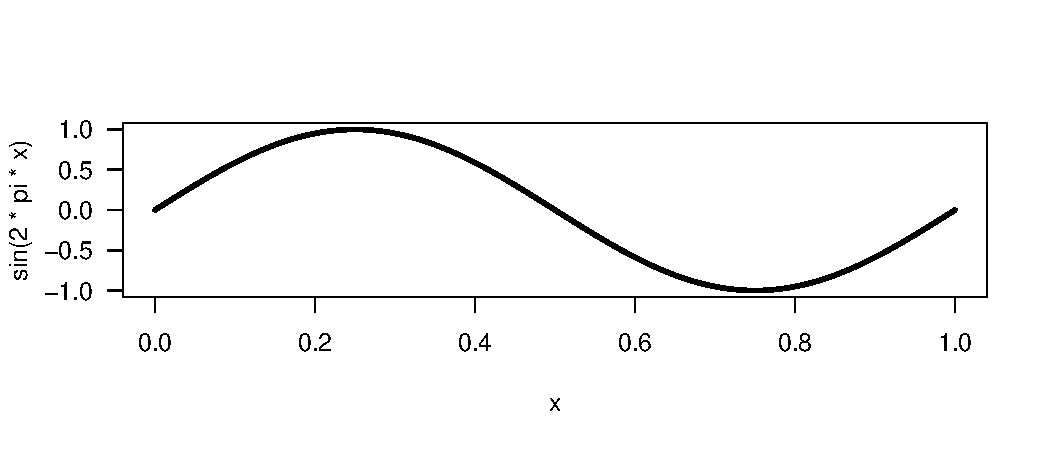
\includegraphics[width=\maxwidth]{figure/example.figure-1} 
\end{knitrout}
  \end{center}
  \caption{This figure illustrates \cref{eq:everything}.}
  \label{fig:everything}
\end{figure}

Note that $\sqrt{2\pi}=2.5066283$ as calculated in the
\texttt{example.calculation} chunk above.  You can supress
the chunk in the typeset document with the chunk option
\texttt{echo=FALSE}.

\section{Discussion}\label{sec:discussion}

Everything is explained by \cref{eq:everything,fig:everything}.

\section*{Acknowledgements}

DJDE was supported by an NSERC Discovery Grant.

\bibliography{ms}
\bibliographystyle{vancouver}

%%\input{mstables}

%%\FloatBarrier

%%\input{msfigures}

\appendix

\section{To Do}\label{app:ToDo}

\begin{itemize}
\item appendices
\item tables
\item Rnw
\item journal templates
\end{itemize}

\end{document}
